% Created 2025-02-16 dom 04:47
% Intended LaTeX compiler: pdflatex
\documentclass[11pt]{article}
\usepackage[utf8]{inputenc}
\usepackage[T1]{fontenc}
\usepackage{graphicx}
\usepackage{longtable}
\usepackage{wrapfig}
\usepackage{rotating}
\usepackage[normalem]{ulem}
\usepackage{amsmath}
\usepackage{amssymb}
\usepackage{capt-of}
\usepackage{hyperref}
\usepackage{minted}
\renewcommand*{\contentsname}{Contenidos}

\usepackage{parskip}
\usepackage[utf8]{inputenc} %% For unicode chars
\usepackage{placeins}
\usepackage[margin=1.40cm]{geometry}
\usepackage[T1]{fontenc}
\usepackage{mathpazo}
\linespread{1.05}
\usepackage[scaled]{helvet}
\usepackage{courier}
\hypersetup{colorlinks=true,linkcolor=blue}
\RequirePackage{fancyvrb}
\DefineVerbatimEnvironment{verbatim}{Verbatim}{fontsize=\small,formatcom = {\color[rgb]{0.5,0,0}}}
\usepackage{mdframed}
\BeforeBeginEnvironment{minted}{\begin{mdframed}}
\AfterEndEnvironment{minted}{\end{mdframed}}
\setcounter{secnumdepth}{3}
\date{}
\title{API REST Con Laravel 9 y 10}
\hypersetup{
 pdfauthor={},
 pdftitle={API REST Con Laravel 9 y 10},
 pdfkeywords={},
 pdfsubject={},
 pdfcreator={Emacs 28.1 (Org mode 9.6.17)}, 
 pdflang={Spanish}}
\begin{document}

\maketitle
\setcounter{tocdepth}{3}
\tableofcontents

\setlength\parindent{10pt}

\section{API REST con Laravel}
\label{sec:org7a719ac}
Vamos a ver las posibilidades de escribir una \texttt{API REST} con
Laravel 10. Podemos hacer un \texttt{CRUD} como hemos hecho antes con el
blog. Nos daremos cuenta de que, al final, nos va a quedar algo mucho
más sencillo, puesto que no tendremos vistas ni plantillas, ni
componentes... Sólo \textbf{rutas}, y \textbf{puntos de acceso} —=endpoints=—.

\subsection{API en pocas palabras}
\label{sec:orgafbf7f5}
Una \textbf{Interfaz de Programación de Aplicaciones} permite a dos sistemas
comunicarse uno con otro. Proporciona el lenguaje y el contrato de
como interactuan los dos sistemas. Cada \texttt{API} tiene documentación y
especificaciones que determinan cómo se puede transferir la
información.

Las \texttt{API} (WEB) generalmente se clasifican como \texttt{SOAP} o \texttt{REST} y
ambas se usan para acceder a los servicios web.

\texttt{SOAP} se basa únicamente en \texttt{XML} para proporcionar servicios de
mensajería, mientras que \texttt{REST} ofrece un método más ligero, utilizando
direcciones \texttt{URL} en la mayoría de los casos para recibir o enviar
información.

Vamos a crear \texttt{APIs REST}.

Para aprovechar al máximo las \texttt{API}, las empresas las usan para:
\begin{itemize}
\item Integrarse con \texttt{API} de terceros.
\item Para uso interno.
\item Para exponerla para uso externo.
\end{itemize}



\page


\subsubsection{¿Que es un EndPoint?}
\label{sec:orgbce42ca}
Brevemente un endPoint es un extremo de un canal de
comunicación. Cuando una API interactúa con otro sistema, los puntos
de contacto de esta comunicación se consideran endpoints.

Cuando una API solicita información de una aplicación web o un
servidor web, recibirá una respuesta. El lugar donde las \texttt{API} envían
solicitudes y donde vive el recurso se denomina \texttt{endpoint}.

Para las \texttt{API}, un \texttt{endpoint} puede incluir una \texttt{URL} de un
\emph{servidor}. Cada \texttt{endpoint} es la ubicación desde la cual las API pueden
acceder a los recursos que necesitan para llevar a cabo su función.

\subsection{Laravel Sail}
\label{sec:org1e712c0}
Vamos a usar de nuevo \texttt{Laravel Sail}, que para montar un entorno de
desarrollo es de lo más cómodo y fácil.

Laravel Sail es una interfaz de línea de comandos liviana para
interactuar con el entorno de desarrollo \texttt{Docker} de
\texttt{Laravel}. Proporciona un excelente punto de partida para crear una
aplicación Laravel usando \texttt{PHP}, \texttt{MySQL} y \texttt{Redis} sin requerir
experiencia previa en \texttt{Docker}.

\texttt{Sail} en esencia es un archivo \texttt{docker-compose.yml} y el script sail
que se almacena en la raíz de tu proyecto.

El archivo \texttt{docker-compose.yml} define una variedad de contenedores de
\texttt{Docker}.

\texttt{Sail} es automáticamente instalado con todas las aplicaciones nuevas de
\texttt{Laravel}.


\section{Aplicación Artículos con imágenes (blog con entradas de texto y/o imágenes)}
\label{sec:orgc58cf27}
Al crear una nueva aplicación Laravel a través de Sail, puedes elegir
qué servicios deben configurarse en el archivo docker-compose.yml de
tu nueva aplicación.

Ejemplo:
\begin{minted}[]{bash}
curl -s "https://laravel.build/laravel10-api?with=mysql,redis" | bash
\end{minted}

En el ejemplo anterior se va a instalar mysql y redis, si no
especificas qué servicios quieres por defecto se instala el siguiente
stack: mysql, redis, meilisearch, mailhog y selenium.

Por defecto los comando sail son invocados desde vendor/bin/sail:
\begin{minted}[]{bash}
cd laravel10-api && ./vendor/bin/sail up
\end{minted}

Para evitar escribir repetidamente vendor/bin/sail podemos definir un
alias para invocar comandos de sail más fácilmente:
\begin{minted}[]{bash}
alias sail='bash vendor/bin/sail'
\end{minted}

\subsection{Iniciar y detener Sail}
\label{sec:orgfbf1b57}
Antes de iniciar Sail, debes asegurarte que no hay otros servicios de
bases de datos o servidores web corriendo en tu máquina local ya que
esto puede arrojar errores al ejecutar Sail.

Para iniciar todos los contenedores Docker definidos en el archivo
docker-compose.yml, debes ejecutar el comando up:
\begin{minted}[]{bash}
sail up
\end{minted}

La primera vez que corras Sail up, los contenedores serán construidos
en tu máquina; esto puede tomar varios minutos pero después los
subsecuentes inicios Sail comenzará mucho más rápido.

Para iniciar los contenedores en modo background deberías ejecutar
sail en modo “detached”:
\begin{minted}[]{bash}
sail up -d
\end{minted}

Una vez que se han iniciado los contenedores Docker de la aplicación
puedes acceder con tu navegador web en la dirección: \url{http://localhost}.

\subsection{Rutas, modelos, migraciones y controllers}
\label{sec:orgf77c039}
\begin{itemize}
\item Rutas:
\label{sec:org11dd9df}
Las rutas son el punto de entrada de tu aplicación web; sin estas no
se podría interactuar con el usuario final.

\item Las peticiones HTTP:
\label{sec:org4997572}
A veces son llamados HTTP verbs. Son un conjunto de métodos de
petición para indicar que se desea realizar para un recurso
determinado.
\begin{itemize}
\item GET: solicita un recurso (o lista de recursos).
\item HEAD: pide una respuesta idéntica a la de una petición GET, pero
sin el cuerpo de la respuesta.
\item POST: crea un recurso.
\item PUT: modifica un recurso.
\item DELETE: borra un recurso.
\item OPTIONS: describe las opciones de comunicación para el recurso destino.
\item PATCH: es utilizado para aplicar modificaciones parciales a un recurso.
\end{itemize}

\item Definición de rutas:
\label{sec:org0b7ff96}
Hay varios archivos donde puede definir las rutas; estos se encuentran
en el directorio \texttt{routes}. Nosotros vamos a trabajar con el archivo
\texttt{api.php} dentro del directorio mencionado.

La forma más simple de definir una ruta es emparejando un «path» con
una función anónima \texttt{lambda} (o closure, como les gusta a muchos decir
hoy en día), como se muestra a continuación:
\begin{minted}[]{php}
<?php
Route::get('/', function(){
    return "Hello world";
});
\end{minted}

Aquí la ruta \texttt{localhost/api/} muestra el mensaje: "Hello world".

Lo siguiente es continuar con el modelo, la migración y el controlador.
\end{itemize}

\subsection{Modelos}
\label{sec:org934d3a0}
Para este caso vamos a crear un modelo llamado \texttt{Post} que guardará
información sobre las fotos que queramos con un título y una
descripción. Para ello lanzamos el siguiente comando:
\begin{minted}[]{bash}
sail artisan make:model Post -m
\end{minted}

Al añadir el parámetro \texttt{-m}, le estamos indicando que además del modelo
queremos que cree el archivo de migración para la base de datos.

Una vez creado el modelo, vamos a la carpeta \texttt{database/migrations},
dentro debemos tener un nuevo archivo que como prefijo tendrá la fecha
actual (fecha de la creación de la migración) más
\_create\_posts\_table.php. Este archivo contendrá la información para
crear la tabla posts dentro de nuestra base de datos. Así que para
añadir las columnas que necesitamos, lo abrimos y sustituimos el
contenido del método up por el siguiente:

\begin{minted}[]{php}
<?=
public function up()
{
    Schema::create('posts', function (Blueprint $table) {
        $table->id();
        $table->foreignId('user_id')->constrained();
        $table->string('title');
        $table->string('image');
        $table->mediumText('description');
        $table->timestamps();
    });
}
\end{minted}


Como comenté antes, añadimos los campos para guardar el título, la
imagen y la descripción. También generamos la relación con la tabla de
usuarios para saber de qué usuario es el post. El método \texttt{id()} creará
el campo para la clave primaria y el método \texttt{timestamps()} genera dos
campos para guardar la fecha de creación y la fecha de la última
actualización.

Ahora debemos abrir el archivo \texttt{app/Models/Post.php} y dentro de la
clase, añadiremos el siguiente código de tal forma que el archivo nos
debería quedar algo así:
\begin{minted}[]{php}
<?php

namespace App\Models;

use Illuminate\Database\Eloquent\Factories\HasFactory;
use Illuminate\Database\Eloquent\Model;

class Post extends Model
{
    use HasFactory;

    /**
     * Get the user record associated with the post.
     */
    public function user()
    {
        return $this->belongsTo(User::class);
    }
}
\end{minted}


Con el método \texttt{user} podremos asociar un usuario con el post y podremos
acceder a los datos del usuario cuando recorramos nuestros posts.

Por último, lanzamos el siguiente comando para crear la tabla en la
base de datos:
\begin{minted}[]{bash}
sail artisan migrate
\end{minted}

\subsection{Autenticación con token JWT}
\label{sec:orgd42548d}
El siguiente paso es instalar la dependencia de JWT vía composer, para
ello solo debemos lanzar el siguiente comando:
\begin{minted}[]{bash}
sail composer require tymon/jwt-auth:*
\end{minted}

\subsubsection{Configuración}
\label{sec:org935c616}
Una vez instalado, debemos abrir el archivo \texttt{config/app.php}. Ahí
veremos que retorna un array enorme. Pues bien, debemos ir a la clave
\texttt{providers} y añadir la siguiente línea:
\begin{minted}[]{php}
<?=
Tymon\JWTAuth\Providers\LaravelServiceProvider::class,
\end{minted}

De tal forma que quedaría algo así:
\begin{minted}[]{php}
<?=
'providers' => [

        /*
         * Laravel Framework Service Providers...
         */
        .
        .
        .
        Illuminate\Validation\ValidationServiceProvider::class,
        Illuminate\View\ViewServiceProvider::class,
        Tymon\JWTAuth\Providers\LaravelServiceProvider::class,
        .
        .
        .
],
\end{minted}

Al añadirlo en esta lista, el servicio de \texttt{JWT} se cargará
automáticamente cada vez que un usuario haga una petición a nuestra
API.

Una vez hecho esto, deberemos crear un archivo llamado \texttt{config/jwt.php},
para ello, solo debemos lanzar el siguiente comando y este lo creará
automáticamente:
\begin{minted}[]{bash}
sail artisan vendor:publish --provider="Tymon\JWTAuth\Providers\LaravelServiceProvider"
\end{minted}

Una vez creado, lanzaremos el siguiente comando para crear una
variable de entorno con una \texttt{clave} para JWT. Lanzamos el siguiente
comando y listo[1]:
\begin{minted}[]{bash}
sail artisan jwt:secret
\end{minted}

Ahora deberemos modificar la forma en la que nos autenticamos por
defecto en Laravel así que lo queremos hacer es abrir el archivo
\texttt{config/auth.php} y sustituir unas claves y valores por los siguientes:
\begin{minted}[]{php}
<?=
    .
    .
    .
    'defaults' => [
        'guard' => 'api',
        'passwords' => 'users',
    ],
    .
    .
    .
    'guards' => [
        'api' => [
            'driver' => 'jwt',
            'provider' => 'users',
        ],
    ],
\end{minted}

En la clave \texttt{defaults} lo que hacemos es sustituir \texttt{guard} con valor \texttt{web}
por \texttt{api}, ya que el tipo de login que vamos a usar va a ser el de API.

En la clave \texttt{guards}, cambiamos la clave \texttt{web} por \texttt{api}, ya que no la
necesitamos y en API le diremos que vamos a usar \textbf{el driver de JWT}.

\subsubsection{Modelo}
\label{sec:org4f0bf7c}
Una vez hecho esto, deberemos editar el modelo \texttt{User.php} que ya viene
por defecto en Laravel, asi que abrimos el archivo \texttt{app/Models/User.php}
y reemplazamos su contenido por el siguiente:
\begin{minted}[]{php}
<?php

namespace App\Models;

use Illuminate\Database\Eloquent\Factories\HasFactory;
use Tymon\JWTAuth\Contracts\JWTSubject;
use Illuminate\Notifications\Notifiable;
use Illuminate\Foundation\Auth\User as Authenticatable;

class User extends Authenticatable implements JWTSubject
{
    use Notifiable;
    use HasFactory;

    // Rest omitted for brevity

    /**
     * Get the identifier that will be stored in the subject claim of the JWT.
     *
     * @return mixed
     */
    public function getJWTIdentifier()
    {
        return $this->getKey();
    }

    /**
     * Return a key value array, containing any custom claims to be added to the JWT.
     *
     * @return array
     */
    public function getJWTCustomClaims()
    {
        return [];
    }
}
\end{minted}

\subsubsection{Controlador}
\label{sec:org47b7a03}
Para gestionar las peticiones de login, necesitaremos crear un
controlador que se encargue de la autenticación. Para crearlo,
lanzamos el siguiente comando:
\begin{minted}[]{bash}
sail  artisan make:controller Api/V1/AuthController
\end{minted}

De esta forma, crearemos el controlador para gestionar la
autenticación en la ruta
\texttt{app/Http/Controllers/Api/V1/AuthController.php}. Una vez creado,
añadiremos el siguiente código:
\begin{minted}[]{php}
<?php

namespace App\Http\Controllers\Api\V1;

use App\Http\Controllers\Controller;

class AuthController extends Controller
{
    /**
     * Create a new AuthController instance.
     *
     * @return void
     */
    public function __construct()
    {
        $this->middleware('auth:api', ['except' => ['login']]);
    }

    /**
     * Get a JWT via given credentials.
     *
     * @return \Illuminate\Http\JsonResponse
     */
    public function login()
    {
        $credentials = request(['email', 'password']);

        if (! $token = auth()->attempt($credentials)) {
            return response()->json(['error' => 'Unauthorized'], 401);
        }

        return $this->respondWithToken($token);
    }

    /**
     * Get the authenticated User.
     *
     * @return \Illuminate\Http\JsonResponse
     */
    public function me()
    {
        return response()->json(auth()->user());
    }

    /**
     * Log the user out (Invalidate the token).
     *
     * @return \Illuminate\Http\JsonResponse
     */
    public function logout()
    {
        auth()->logout();

        return response()->json(['message' => 'Successfully logged out']);
    }

    /**
     * Refresh a token.
     *
     * @return \Illuminate\Http\JsonResponse
     */
    public function refresh()
    {
        return $this->respondWithToken(auth()->refresh());
    }

    /**
     * Get the token array structure.
     *
     * @param  string $token
     *
     * @return \Illuminate\Http\JsonResponse
     */
    protected function respondWithToken($token)
    {
        return response()->json([
            'access_token' => $token,
            'token_type' => 'bearer',
            'expires_in' => auth()->factory()->getTTL() * 60
        ]);
    }
}
\end{minted}
Este código se encargará de gestionar las distintas rutas que
utilizaremos para todo el proceso de autenticación.

\textbf{Nota}:
\begin{mdframed}
Para las pruebas podemos cambiar el campo \texttt{expires\_in}, para no tener
que generar un nuevo token cada dos por tres.
\end{mdframed}

\subsubsection{Rutas}
\label{sec:org89d6ead}
El siguiente paso que haremos, será configurar las rutas así abrimos
el archivo \texttt{routes/api.php} y sustituimos su contenido por el siguiente:
\begin{minted}[]{php}
<?php

use Illuminate\Support\Facades\Route;

Route::group([
    'middleware' => 'api',
    'prefix' => 'v1/auth'

], function ($router) {
    Route::post('login', [\App\Http\Controllers\Api\V1\AuthController::class,
                 'login'])->name('login');
    Route::post('logout', [\App\Http\Controllers\Api\V1\AuthController::class,
                  'logout'])->name('logout');
    Route::post('refresh', [\App\Http\Controllers\Api\V1\AuthController::class,
                 'refresh'])->name('refresh');
    Route::post('me', [\App\Http\Controllers\Api\V1\AuthController::class,
                 'me'])->name('me');
});
\end{minted}


Como podéis ver, la dependencia de \texttt{JWT} en Laravel nos crea varias
rutas aunque en nuestro caso sólo utilizaremos la ruta de login para
obtener el token de acceso.

También, todas nuestras rutas tendrán un \emph{prefijo} \texttt{v1/auth}, de esta
forma si luego trabajamos con otra versión, podremos separar como
hacer la autenticación de una versión a otra.

\subsubsection{Configuración de la BD}
\label{sec:orgc6d02fc}
Como siempre, deberemos editar el archivo \texttt{.env} para añadir las
conexiones a la base de datos así que lo abrimos y añadimos la
configuración a nuestra \texttt{BD}. Nos vale con lo que sail hace, nada que
tocar.

Normalmente con Sail no hay que crear la BD, pero a veces se tiene que
crear la base de datos con el nombre que queráis en vuestro cliente de
MySQL para que todo funcione correctamente.

El siguiente paso es crear unos cuantos usuarios para probar que todo
funciona correctamente. Para ello, vamos al archivo
\texttt{database/seeders/DatabaseSeeder.php} y descomentamos la línea para
crear los usuarios. De esta forma podremos crearlos automáticamente
cuando lancemos la migración de las tablas a la base de datos.
\begin{minted}[]{php}
<?=
public function run()
{
    \App\Models\User::factory(10)->create();
}
\end{minted}

Una vez hecho esto, vamos a crear los usuarios y las tablas en la base
de datos. Para ello lanzamos el siguiente comando:
\begin{minted}[]{bash}
sail artisan migrate --seed
\end{minted}

\subsection{CRUD}
\label{sec:org2237f21}
Ahora que ya tenemos el modelo, es hora de ponerse manos a la obra con
el CRUD, así que lo primero que vamos a hacer es crear el controlador
con el siguiente comando:
\begin{minted}[]{bash}
sail php artisan make:controller Api/V1/PostController --api --model=Post
\end{minted}

Al igual que el controlador de autenticación, \texttt{PostController} será
guardado dentro de la carpeta V1 para poder separar futuras versiones
de la \texttt{API}. El parámetro \texttt{-{}-{}api} creará automáticamente los métodos del
\texttt{CRUD} y \texttt{-{}-{}model=Post} le indicará que este controlador trabajará con los
datos del modelo \texttt{Post}.

Ahora que ya tenemos el controlador, vamos a generar las rutas así que
vamos al archivo \texttt{routes/api.php} y añadimos la siguiente línea:

\begin{minted}[]{php}
<?=
//en una sola línea
Route::apiResource('v1/posts',
                  App\Http\Controllers\Api\V1\PostController::class)
                   ->middleware('api');
\end{minted}

Con esta simple línea crearemos todas las rutas con las que podremos
acceder a los cinco métodos de \texttt{PostController} que podrán realizar las
siguientes acciones:

\begin{itemize}
\item Mostrar un listado de todos los post con las fotos.
\item Mostrar un post en concreto por el id.
\item Crearlas.
\item Actualizarlas
\item Eliminarlas.
\end{itemize}

Para ver las rutas generadas, podéis lanzar el siguiente comando:
\begin{minted}[]{bash}
sail artisan route:list
\end{minted}

Ahora tenemos las rutas, pero nos falta controlar que los \texttt{endpoints}
para la \emph{creación, actualización y borrado} necesiten de un usuario
autenticado para poder utilizarlos. Para añadir este control, debemos
ir al archivo \texttt{app/Http/Controllers/Api/V1/PostController.php} y en él
crearemos el constructor de la clase en el que añadiremos el siguiente
código:
\begin{minted}[]{php}
public function __construct()
{
    $this->middleware('auth:api', ['except' => ['index', 'show']]);
}
\end{minted}

Con esta línea le diremos a Laravel que, a excepción de los métodos
\texttt{index} y \texttt{show}, los demás necesitarán pasar por el middleware
\texttt{auth:api}, el cual se encargará de \emph{validar} el \texttt{token} que pasemos por
la cabecera.

\subsubsection{Creación}
\label{sec:orgc483b0c}
Ahora que ya tenemos las rutas y el controlador es hora de darle
vidilla a nuestra \texttt{API}. Para ello, lo primero que haremos será
habilitar la funcionalidad para añadir nuevos posts para más adelante
poder probar los endpoints para listar todos los post y el post por
id.

Lo primero que vamos a hacer es crear un objeto \texttt{Request}. Esta
funcionalidad la utilizaremos para validar los datos que nos envíe el
usuario. Para crear la request lanzamos el siguiente comando:
\begin{minted}[]{bash}
sail artisan make:request V1/PostRequest
\end{minted}

Al lanzar este comando nos creará un archivo dentro de la ruta
\texttt{app/Http/Requests/V1/PostRequest.php}. Pues bien, lo que vamos a hacer
ahora es abrir ese archivo y sustituir su contenido por el siguiente:
\begin{minted}[]{php}
<?php

namespace App\Http\Requests\V1;

use Illuminate\Foundation\Http\FormRequest;
use Illuminate\Support\Facades\Auth;

class PostRequest extends FormRequest
{
    /**
     * Determine if the user is authorized to make this request.
     *
     * @return bool
     */
    public function authorize()
    {
        return Auth::check();
    }

    /**
     * Get the validation rules that apply to the request.
     *
     * @return array
     */
    public function rules()
    {
        return [
            'title' => 'required|max:70',
            'image' => 'required|image|max:1024',
            'description' => 'required|max:2000',
        ];
    }
}
\end{minted}

Este archivo tiene dos métodos, el primero, el método \texttt{authorize} que
sólo \textbf{permitirá realizar la petición si el usuario está
autenticado}. Para ello utiliza el método \texttt{check} de la clase \texttt{Auth}
que devuelve \texttt{true} si el usuario que realiza la petición está
autenticado, y si no, devolverá \texttt{false}. En caso de no estar autenticado
retornará el \texttt{error 401 unauthorized}.

El segundo método es el método \texttt{rules}. En este método \textbf{validaremos} los
datos que nos debe enviar el usuario que son el título, la imagen y la
descripción. Como podéis ver, retorna un array con formato clave valor
en el que cada clave es el campo a enviar y su valor son las distintas
reglas que debe cumplir para ser validado separadas por |. Si no
cumple alguna de estas reglas, Laravel devolverá un error.

Dicho esto vamos a explicar las reglas que vamos a utilizar:

La regla \texttt{required} indicará que el campo es obligatorio.

En \texttt{title}, \texttt{max:70} indicará el número máximo de caracteres que podrá
enviar un usuario para asignar un título.

En \texttt{image}, añadimos la regla \texttt{image} que indica que vamos a enviar un
fichero de tipo imagen. En este caso, \texttt{max:1024} indicará que el tamaño
máximo de una imagen será de \emph{1024 KB}.

En \texttt{description} al igual que en title añadimos la regla max esta vez
con un límite de \emph{2000 caracteres}.

Aparte de estas hay muchas más reglas, para verlas podéis hacerlo
pinchando en el \href{https://laravel.com/docs/10.x/validation}{siguiente enlace}.

El siguiente paso que vamos a realizar es añadir la funcionalidad para
poder \emph{crear post}. Para ello abrimos el
archivo \texttt{app/Http/Controllers/Api/V1/PostController.php} e importamos
las clases \texttt{PostRequest} y \texttt{Auth}, aparte, añadimos el siguiente código en
el método \texttt{store} y creamos el método \texttt{update} que usaremos para guardar
las imágenes.
\begin{minted}[]{php}
<?php

namespace App\Http\Controllers\Api\V1;

use App\Http\Controllers\Controller;
use App\Models\Post;
use Illuminate\Http\Request;
use App\Http\Requests\V1\PostRequest;
use Illuminate\Support\Facades\Auth;

class PostController extends Controller
{
...
    /**
     * Store a newly created resource in storage.
     *
     * @param  App\Http\Requests\V1\PostRequest $request
     * @return \Illuminate\Http\Response
     */
    public function store(PostRequest $request)
    {
        $request->validated();

        $user = Auth::user();

        $post = new Post();
        $post->user()->associate($user);
        $url_image = $this->upload($request->file('image'));
        $post->image = $url_image;
        $post->title = $request->input('title');
        $post->description = $request->input('description');

        $res = $post->save();

        if ($res) {
            return response()->json(['message' => 'Post create succesfully'], 201);
        }
        return response()->json(['message' => 'Error to create post'], 500);
    }

    private function upload($image)
    {
        $path_info = pathinfo($image->getClientOriginalName());
        $post_path = 'images/post';

        $rename = uniqid() . '.' . $path_info['extension'];
        $image->move(public_path() . "/$post_path", $rename);
        return "$post_path/$rename";
    }
...
\end{minted}

Una vez hecho esto vamos a explicar que es lo que hace el método
\texttt{store}.

Lo primero que hacemos es validar los datos que nos envía el usuario,
para ello lanzamos el método \texttt{validated()} del objeto \texttt{\$request} y este
comprobará que se cumplen las reglas que creamos en la clase
\texttt{PostRequest}.

El siguiente paso es obtener el usuario y crear un objeto de tipo
\texttt{post} para guardar la información. \textbf{Asociamos el usuario al post} y
nos valemos del método \textbf{upload} para guardar la imagen en la carpeta
pública de Laravel y nos retornará su \texttt{url}, de esta forma podremos
guardar su ruta en la bbdd y visualizarla más adelante.

Añadimos también el título y la descripción y usamos el método \texttt{save}
del objeto \texttt{\$post} para guardar los cambios. Si todo ha ido bien
retornará \texttt{true} y enviaremos al usuario un \emph{mensaje diciendo que todo ha
ido bien}, si no, le diremos al usuario que \emph{hemos tenido un error} y nos
tocará revisar.

Ahora que ya lo tenemos montado es hora de probarlo. Usaremos \href{https://insomnia.rest/}{Insomnia}
o \href{https://www.postman.com/product/rest-client/}{Postman}, pero podéis utilizar la herramienta que más os guste.

Primero deberemos generar el \texttt{token JWT} para poder autenticarnos: En
\texttt{Insomnia} (o \texttt{Postman}), creamos una petición tipo \texttt{POST} contra la \texttt{url}
\texttt{localhost/api/v1/auth/login}
\begin{center}
\includegraphics[width=.9\linewidth]{LoginObtenciónDelToken.png}
\end{center}

Una vez hecho esto lanzaremos una petición a la siguiente
url \texttt{http://localhost/api/v1/posts}. Esta petición deberá ser de
tipo \texttt{POST} y en ella deberemos enviar los parámetros \texttt{title}, \texttt{image} y
\texttt{description}. También tenemos que enviar las siguientes cabeceras para
que funcione correctamente:

\begin{minted}[]{html}
Content-type: multipart/form-data;
Authorization: Bearer <my-token>
Accept: application/json
\end{minted}

El \texttt{Bearer Token} lo podemos poner en la pestaña de \texttt{Auth} donde
seleccionaremos \texttt{Bearer token} y pegamos el \texttt{token JWT} obtenido
anteriormente.

\begin{center}
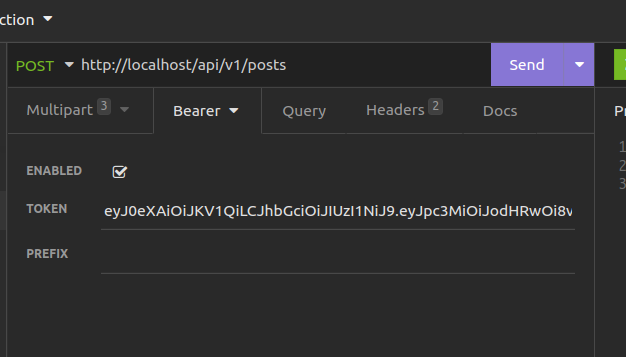
\includegraphics[width=.9\linewidth]{BearerToken.png}
\end{center}

La creación del post la mandamos en el cuerpo del mensaje —body—.

\begin{center}
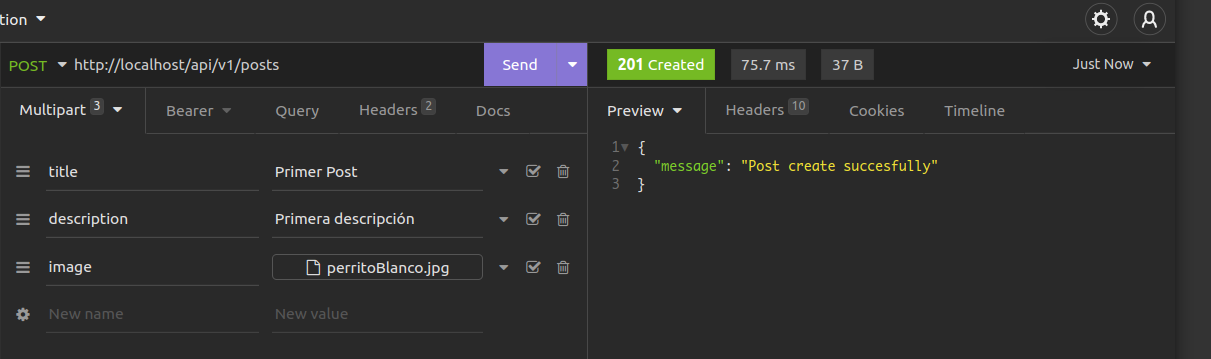
\includegraphics[width=.9\linewidth]{PrimerPost.png}
\end{center}

El resto de cabeceras las añadimos en Headers:

\begin{center}
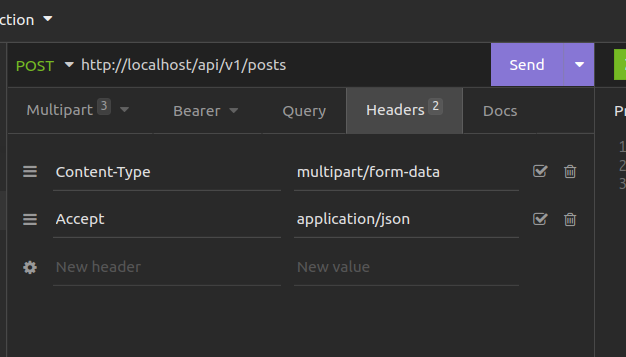
\includegraphics[width=.9\linewidth]{RestoCabeceras.png}
\end{center}


\subsubsection{Lectura}
\label{sec:org3842115}
Para mostrar datos, Laravel provee una clase intermediaria para poder
modificar la respuesta, lo que nos permitiría ocultar \texttt{ids}, mostrar lo
que queramos... Son los recursos —=Resources=—. Primero la creamos:
\begin{minted}[]{bash}
sail artisan make:resource V1/PostResource
\end{minted}

Este comando generará un archivo en la ruta
\texttt{app/Http/Resources/V1/PostResource.php}. Por defecto tiene un método
llamado \texttt{toArray} que recibe una \texttt{Request} (que en este caso sería el
\texttt{post}) y lo convierte en array, pero nosotros vamos a cambiar levemente
el funcionamiento para modificar los datos que queremos mostrar y como
mostrarlos. Abrimos el archivo y sustituimos el contenido del método
\texttt{toArray} por el siguiente:
\begin{minted}[]{php}
<?=
public function toArray($request)
{
    return [
        'id' => $this->id,
        'title' => $this->title,
        'description' => $this->description,
        'photo' => url($this->image),
        'author' => [
            'name' => $this->user->name,
            'email' => $this->user->email,
        ],
        'created_at' => $this->created_at
    ];
}
\end{minted}

Cuando creemos un objeto de tipo \texttt{PostResource}, este podrá recibir un
\texttt{post} o una \texttt{colección de posts}. Al llamar al campo \texttt{toArray}, recorrerá
los posts y podremos acceder a sus campos gracias a \texttt{\$this}. De esta
forma hemos podido realizar las siguientes modificaciones:
\begin{itemize}
\item Ya no mostramos el campo \texttt{updated\_at}.
\item Hemos renombrado el campo \texttt{image} por \texttt{photo}, además añadimos la
\texttt{url} y no sólo donde está almacenada en el proyecto. Esto lo hacemos
porque sin ello no podríamos ver la imagen.
\item Hemos añadido el \texttt{nombre de usuario} y el \texttt{email} del autor del \texttt{post}.
\end{itemize}

Ahora que ya tenemos el \texttt{Resource} configurado es hora de utilizarlo,
para ello abrimos el archivo \texttt{PostController.php}, añadimos la clase
\texttt{PostResource} y modificamos los métodos \texttt{index} y \texttt{show} con el siguiente
código:
\begin{minted}[]{php}
<?php

...
use App\Http\Resources\V1\PostResource;

class PostController extends Controller
{
    ...
    /**
     * Display a listing of the resource.
     *
     * @return \Illuminate\Http\Response
     */
    public function index()
    {
        return PostResource::collection(Post::latest()->paginate());
    }
    ...
    public function show(Post $post)
    {
         return new PostResource($post);
    }
    ...
\end{minted}

El método \texttt{index} se encargará de \emph{retornar} todos los \texttt{posts}
disponibles. Al utilizar el método \texttt{collection} de \texttt{PostResource} y al
devolver los posts páginados con el modelo \texttt{Post}, obtendremos un
listado de los 15 últimos posts. Además nos mostrará los \emph{links a
sucesivas páginas de posts} y una clave \texttt{meta} con información como el
número total de posts, posts por página, etc. Vamos que nos da mucha
información sin hacer prácticamente nada.

Para obtener el \emph{listado de posts} sólo tendremos que lanzar una
petición de tipo \texttt{GET} a la siguiente url: \texttt{localhost/api/v1/auth/posts}.

Este endpoint nos devolverá el siguiente \texttt{json} (cambiando mis posts por
los vuestros):
\begin{minted}[]{javascript}
{
        "data": [
                {
                        "id": 1,
                        "title": "Primer Post",
                        "description": "Primera descripción",
                        "photo": "http:\/\/localhost\/images\/post\/639311daf18ce.jpg",
                        "author": {
                                "name": "Test User",
                                "email": "test@example.com"
                        },
                        "created_at": "2022-12-09T10:45:46.000000Z"
                }
        ],
        "links": {
                "first": "http:\/\/localhost\/api\/v1\/posts?page=1",
                "last": "http:\/\/localhost\/api\/v1\/posts?page=1",
                "prev": null,
                "next": null
        },
        "meta": {
                "current_page": 1,
                "from": 1,
                "last_page": 1,
                "links": [
                        {
                                "url": null,
                                "label": "&laquo; Previous",
                                "active": false
                        },
                        {
                                "url": "http:\/\/localhost\/api\/v1\/posts?page=1",
                                "label": "1",
                                "active": true
                        },
                        {
                                "url": null,
                                "label": "Next &raquo;",
                                "active": false
                        }
                ],
                "path": "http:\/\/localhost\/api\/v1\/posts",
                "per_page": 15,
                "to": 1,
                "total": 1
        }
}
\end{minted}

El método \texttt{show} se encargará de mostrarnos un único post enviando el
\texttt{id} por la \texttt{url}. Este método crea un objeto de tipo \texttt{PostResource} y
recibe el objeto post en el constructor.

Para realizar la petición debemos lanzar una petición de tipo \texttt{GET} a la
siguiente url \texttt{http://localhost:8000/api/v1/posts/1}  sustituyendo el id
del post que queráis mostrar por el \textbf{1} que es que quiero visualizar yo:

Esta petición devolverá el siguiente resultado:
\begin{minted}[]{javascript}
{
        "data": {
                "id": 1,
                "title": "Primer Post",
                "description": "Primera descripción",
                "photo": "http:\/\/localhost\/images\/post\/639311daf18ce.jpg",
                "author": {
                        "name": "Test User",
                        "email": "test@example.com"
                },
                "created_at": "2022-12-09T10:45:46.000000Z"
        }
}
\end{minted}


\subsubsection{Actualización}
\label{sec:org622f04b}
El siguiente paso es crear la actualización, para ello vamos al
archivo \texttt{PostController.php}, importamos la clase \texttt{Validator} y
modificamos el método \texttt{update} con el siguiente código:
\begin{minted}[]{php}
<?=
...
use Illuminate\Support\Facades\Validator;

class PostController extends Controller
{

    public function update(Request $request, Post $post)
    {
        Validator::make($request->all(), [
            'title' => 'max:191',
            'image' => 'image|max:1024',
            'description' => 'max:2000',
        ])->validate();

        if (Auth::id() !== $post->user->id) {
            return response()->json(['message' => 'You don\'t have permissions'], 403);
        }

        if (!empty($request->input('title'))) {
            $post->title = $request->input('title');
        }
        if (!empty($request->input('description'))) {
            $post->description = $request->input('description');
        }
        if (!empty($request->file('image'))) {
            $url_image = $this->upload($request->file('image'));
            $post->image = $url_image;
        }

        $res = $post->save();

        if ($res) {
            return response()->json(['message' => 'Post update succesfully']);
        }

        return response()->json(['message' => 'Error to update post'], 500);
    }
\end{minted}

Una vez añadido el código vamos a explicar que hace:

\begin{itemize}
\item En este caso, en vez de crear un archivo \texttt{request}, se ha añadido la
validación desde el propio método gracias a la clase \texttt{Validator}. Como
veis solo tenemos que añadir las reglas como en el archivo \texttt{request} y
lanzar el método \texttt{validate()}.
\item El siguiente paso es verificar que el usuario que realiza la
petición es el \emph{propietario del post}. Si no es así \emph{mostraremos un
error}.
\item Después comprobamos que datos ha enviado el usuario y que sólo
modificamos los existentes.
\item Por último guardamos y si todo ha ido bien retornamos un mensaje
afirmativo.
\end{itemize}

\textbf{Importante}:
\begin{mdframed}
Para lanzar la actualización en Laravel \textbf{NO} debemos usar el
método \texttt{PUT} o \texttt{PATCH} en los casos en los que enviemos archivos, ya
que \texttt{PHP} \textbf{NO guarda} la información en la super variable \texttt{\$\_FILES} en una
petición \texttt{PUT} o \texttt{PATCH} y por lo tanto no podremos actualizar este campo
si se da el caso. Tendremos que lanzar una petición de tipo \texttt{POST} y
enviar el parámetro \textbf{\_method: \texttt{PUT}} en la cabecera.
\end{mdframed}

La petición será igual a la que realizamos para pedir un \texttt{POST} en el
que debemos añadir el \texttt{id} del post que queremos actualizar.

Os dejo captura para que lo veáis más claro:
\begin{center}
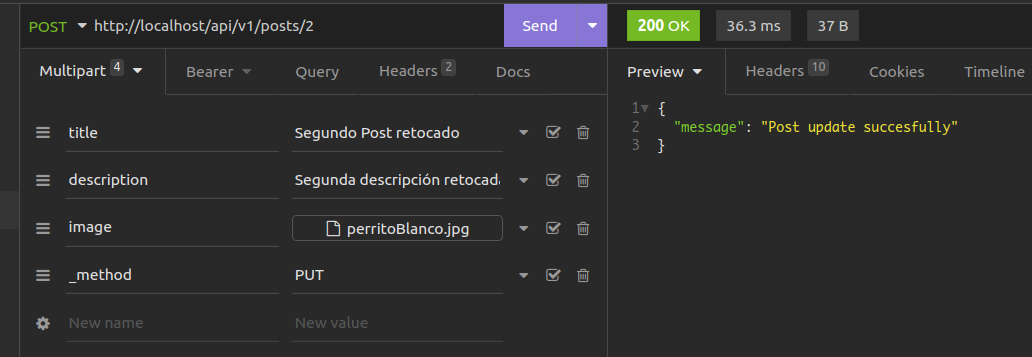
\includegraphics[width=.9\linewidth]{UpdatePost.png}
\end{center}

\subsubsection{Borrado}
\label{sec:org3556602}
Por último vamos a crear la acción de borrado. Volvemos al archivo
\texttt{PostController.php} y modificamos el método \texttt{destroy} por el siguiente
código:
\begin{minted}[]{php}
<?=
public function destroy(Post $post)
{
    if (Auth::id() !== $post->user_id) {
        return response()->json(['message' => 'You are not the owner of this post'], 403);
    }

    // Eliminar la imagen asociada
    $this->deleteImage($post->image);

    $res = $post->delete();
    if ($res) {
        return response()->json(['message' => 'Post deleted successfully'], 200);
    }
    return response()->json(['message' => 'Error to delete post'], 500);
}

private function deleteImage($imagePath)
{
        $fullPath = public_path($imagePath);
        if (file_exists($fullPath)) {
            @unlink($fullPath); // Elimina el archivo
        }
}
\end{minted}

La función \texttt{deleteImage} se encarga de eliminar el archivo de la
imagen del disco.

\begin{itemize}
\item Obtener la ruta completa: Convierte la ruta relativa de la imagen
(\$imagePath) a una ruta completa en el sistema de archivos
(\texttt{\$fullPath = public\_path(\$imagePath)}).
\item Comprobar si el archivo existe: Verifica si el archivo existe en la
ruta especificada (if (file\_exists(\$fullPath))).
\item Eliminar el archivo: Si el archivo existe, lo elimina usando la
función unlink() de PHP (@unlink(\$fullPath)). El operador @ suprime
cualquier error que pueda ocurrir durante la eliminación.
\end{itemize}

En este caso solo debemos lanzar el método \texttt{delete} y listo, nuestro
post habrá sido eliminado.

Para lanzar la petición deberemos utilizar el método \texttt{DELETE} y usar la
siguiente \texttt{url} sustituyendo el número final por el \texttt{id} del post que
queramos eliminar, ejemplo: \texttt{http://localhost:8000/api/v1/posts/1}

\subsection{Control de Errores en la API}
\label{sec:org31bb50a}

En este paso, añadiremos un sistema de control de errores a nuestra
API para mejorar la respuesta en casos de errores como peticiones
inválidas, recursos no encontrados o errores del servidor.

\subsection{2.6.1 Middleware de Manejo de Errores}
\label{sec:org997c330}

Laravel maneja excepciones mediante la clase \texttt{Handler.php}, pero
podemos crear un middleware específico para manejar respuestas de
error de forma más estructurada.

Ejecutamos el siguiente comando para crear un middleware de manejo de
errores:

\begin{minted}[]{bash}
sail artisan make:middleware ApiExceptionHandler
\end{minted}

Luego editamos \texttt{app/Http/Middleware/ApiExceptionHandler.php} y
agregamos lo siguiente:

\begin{minted}[]{php}
namespace App\Http\Middleware;

use Closure;
use Illuminate\Http\JsonResponse;
use Illuminate\Database\Eloquent\ModelNotFoundException;
use Symfony\Component\HttpKernel\Exception\HttpException;
use Throwable;

class ApiExceptionHandler
{
    public function handle($request, Closure $next)
    {
        try {
            return $next($request);
        } catch (ModelNotFoundException $e) {
            return response()->json(['error' => 'Recurso no encontrado'], 404);
        } catch (HttpException $e) {
            return response()->json(['error' => $e->getMessage()], $e->getStatusCode());
        } catch (Throwable $e) {
            return response()->json(['error' => 'Error interno del servidor'], 500);
        }
    }
}
\end{minted}

Registramos el middleware en \texttt{app/Http/Kernel.php} dentro de \texttt{\$middlewareAliases}:

\begin{minted}[]{php}
'api.exception' => \App\Http\Middleware\ApiExceptionHandler::class,
\end{minted}

Ahora podemos aplicar este middleware en nuestras rutas de la API.

\subsection{Manejo de Excepciones en los Controladores}
\label{sec:org2cdc6e7}

En nuestros controladores, podemos lanzar excepciones en caso de
errores. Modificamos \texttt{PostController.php} para añadir un manejo
adecuado en los métodos \texttt{show}, \texttt{update} y \texttt{destroy}.

\begin{minted}[]{php}
use Illuminate\Http\JsonResponse;
use Illuminate\Database\Eloquent\ModelNotFoundException;

public function show(Post $post): JsonResponse
{
    if (!$post) {
        throw new ModelNotFoundException("Post no encontrado");
    }
    return response()->json(new PostResource($post), 200);
}

public function update(Request $request, Post $post): JsonResponse
{
    if (Auth::id() !== $post->user->id) {
        return response()->json(['message' => 'No tienes permisos'], 403);
    }
    // Actualización del post...
}

public function destroy(Post $post): JsonResponse
{
    if (!$post) {
        throw new ModelNotFoundException("Post no encontrado");
    }
    $post->delete();
    return response()->json(['message' => 'Post eliminado'], 200);
}
\end{minted}

\subsection{Validaciones Mejoradas en Requests}
\label{sec:org588a269}

Modificamos \texttt{PostRequest.php} para personalizar los mensajes de error:

\begin{minted}[]{php}
public function messages()
{
    return [
        'title.required' => 'El título es obligatorio.',
        'title.max' => 'El título no puede superar los 70 caracteres.',
        'image.required' => 'La imagen es obligatoria.',
        'image.image' => 'El archivo debe ser una imagen.',
        'description.required' => 'La descripción es obligatoria.',
    ];
}
\end{minted}


\subsubsection{Middleware no intercepta errores al pedir un post inexistente}
\label{sec:org2112ca3}
Laravel lanza una \texttt{ModelNotFoundException} cuando se usa "Route Model
Binding" (\texttt{Post \$post}) y el post no existe. Esto no se capturaba en
el middleware por defecto.

\begin{itemize}
\item Solución:
\label{sec:org8b234ed}
Modificamos \texttt{ApiExceptionHandler.php} para capturar \texttt{ModelNotFoundException}:

\begin{minted}[]{php}
use Illuminate\Database\Eloquent\ModelNotFoundException;

public function handle($request, Closure $next)
{
    try {
        return $next($request);
    } catch (ModelNotFoundException $e) {
        return response()->json(['error' => 'Recurso no encontrado'], 404);
    }
    // Otras capturas de errores...
}
\end{minted}

Después de estos cambios, la API devolverá respuestas JSON más claras
y estructuradas en caso de errores.
\end{itemize}


\subsection{Troubleshooting de Errores Comunes}
\label{sec:org4b245c3}

\subsubsection{"Please provide a valid cache path"}
\label{sec:orgf1d49ca}
Este error ocurre cuando Laravel no puede escribir en la caché debido
a un problema con la ruta de almacenamiento.

\begin{itemize}
\item Solución:
\label{sec:org8e330a3}
Ejecuta estos comandos para limpiar y regenerar la caché:

\begin{minted}[]{bash}
sail artisan config:clear
sail artisan cache:clear
sail artisan config:cache
\end{minted}

Si el problema persiste, asegúrate de que la carpeta
\texttt{storage/framework/cache} existe y tiene los permisos correctos:

\begin{minted}[]{bash}
sail artisan storage:link
chmod -R 775 storage bootstrap/cache
\end{minted}
\end{itemize}

\section{2.7 Próximos Pasos en la API}
\label{sec:orgec7a6d3}

Ahora que hemos implementado un control de errores sólido en nuestra
API de Laravel 10, hay algunos aspectos adicionales que se pueden
mejorar para optimizar su funcionamiento y seguridad.

\subsection{2.7.1 Implementación de Logging de Errores}
\label{sec:org10796bc}

Es recomendable registrar los errores para facilitar la depuración y
el monitoreo del sistema. Podemos hacerlo en \texttt{Handler.php} utilizando
Laravel Logging:

\begin{minted}[]{php}
use Illuminate\Support\Facades\Log;

public function render($request, Throwable $exception)
{
    Log::error('Error en la API', [
        'exception' => $exception,
        'url' => $request->fullUrl(),
        'user' => auth()->user() ? auth()->user()->id : 'guest'
    ]);

    return parent::render($request, $exception);
}
\end{minted}

Esto guardará los errores en \texttt{storage/logs/laravel.log} para su
análisis posterior.

\subsection{2.7.2 Configuración de CORS para Integración con Vue.js}
\label{sec:orgf25338c}

Para permitir que el frontend en Vue.js pueda consumir la API sin
problemas de seguridad, configuramos CORS en \texttt{config/cors.php}:

\begin{minted}[]{php}
return [
    'paths' => ['api/*', 'sanctum/csrf-cookie'],
    'allowed_methods' => ['*'],
    'allowed_origins' => ['http://localhost:5173'], // Ajustar al dominio del frontend
    'allowed_origins_patterns' => [],
    'allowed_headers' => ['*'],
    'exposed_headers' => [],
    'max_age' => 0,
    'supports_credentials' => true,
];
\end{minted}

También agregamos el middleware de CORS en \texttt{app/Http/Kernel.php}:

\begin{minted}[]{php}
protected $middlewareGroups = [
    'api' => [
        \Illuminate\Cors\Middleware\HandleCors::class,
        'throttle:60,1',
        \Illuminate\Routing\Middleware\SubstituteBindings::class,
    ],
];
\end{minted}

Esto permitirá que Vue.js pueda interactuar con la API sin bloqueos
por política de seguridad del navegador.


\subsection{2.7.2b Implementación de Rate Limiting}
\label{sec:org7b891ce}

Para evitar abusos en nuestra API, podemos implementar límites de tasa
en \texttt{app/Http/Kernel.php}:

\begin{minted}[]{php}
protected $middlewareGroups = [
    'api' => [
        'throttle:60,1', // 60 solicitudes por minuto
        \Illuminate\Routing\Middleware\SubstituteBindings::class,
    ],
];
\end{minted}

Esto limitará las solicitudes de un mismo usuario en un período de tiempo.

\subsection{2.7.3 Documentación con OpenAPI (Swagger)}
\label{sec:org8e8c4b2}

Para mejorar la usabilidad de nuestra API, podemos generar
documentación automática con Swagger. Instalamos el paquete:

\begin{minted}[]{bash}
composer require darkaonline/l5-swagger
\end{minted}

Y generamos la documentación con:

\begin{minted}[]{bash}
php artisan l5-swagger:generate
\end{minted}

Ahora los usuarios podrán acceder a
\texttt{http://localhost/api/documentation} para consultar la API.

\subsection{2.7.4 Pruebas Unitarias y de Integración}
\label{sec:org2be9c58}

Añadimos pruebas para asegurar que los errores se manejan
correctamente. Creamos un test:

\begin{minted}[]{bash}
php artisan make:test ApiErrorHandlingTest
\end{minted}

Ejemplo de prueba en \texttt{tests/Feature/ApiErrorHandlingTest.php}:

\begin{minted}[]{php}
public function test_not_found_error()
{
    $response = $this->getJson('/api/v1/posts/9999');
    $response->assertStatus(404)->assertJson(['error' => 'Recurso no encontrado']);
}
\end{minted}

\subsection{2.7.5 Seguridad Adicional: Validación de Payloads con JSON Schema}
\label{sec:orgd4597a8}

Podemos asegurar que las solicitudes cumplen con un esquema
predefinido utilizando el paquete \texttt{justinrainbow/json-schema}:

\begin{minted}[]{bash}
composer require justinrainbow/json-schema
\end{minted}

Y validamos en nuestros controladores:

\begin{minted}[]{php}
use JsonSchema\Validator;

$validator = new Validator;
$validator->validate($request->all(),
 (object)['type' => 'object', 'required' => ['title', 'description']]);
if (!$validator->isValid()) {
    return response()->json(['error' => 'Payload inválido'], 400);
}
\end{minted}

\subsection{2.7.6 Implementación de Roles y Permisos}
\label{sec:orgf245c2f}

Para gestionar permisos en la API, podemos utilizar Laravel \textbf{\textbf{Gates}}
o el paquete \texttt{spatie/laravel-permission}.

\subsubsection{Instalación del paquete de roles y permisos}
\label{sec:org1843da7}

\begin{minted}[]{bash}
composer require spatie/laravel-permission
\end{minted}

Publicamos la configuración y ejecutamos las migraciones:

\begin{minted}[]{bash}
php artisan vendor:publish --provider="Spatie\Permission\PermissionServiceProvider"
php artisan migrate
\end{minted}

\subsubsection{Definir Roles y Permisos}
\label{sec:org43f4456}

En \texttt{App/Models/User.php}, añadimos:

\begin{minted}[]{php}
use Spatie\Permission\Traits\HasRoles;

class User extends Authenticatable
{
    use HasRoles;
}
\end{minted}

En un Seeder, creamos roles y permisos:

\begin{minted}[]{php}
use Spatie\Permission\Models\Role;
use Spatie\Permission\Models\Permission;

Role::create(['name' => 'admin']);
Role::create(['name' => 'editor']);
Role::create(['name' => 'user']);

Permission::create(['name' => 'create post']);
Permission::create(['name' => 'edit post']);
Permission::create(['name' => 'delete post']);

$admin = Role::findByName('admin');
$admin->givePermissionTo(['create post', 'edit post', 'delete post']);
\end{minted}

\subsubsection{Aplicar Permisos en Controladores}
\label{sec:org7f23166}

Podemos restringir el acceso con middleware en \texttt{routes/api.php}:

\begin{minted}[]{php}
Route::middleware(['auth:sanctum', 'role:admin'])->group(function () {
  Route::post('/posts', [PostController::class, 'store']);
  Route::delete('/posts/{post}', [PostController::class, 'destroy']);
});
\end{minted}

O dentro del controlador:

\begin{minted}[]{php}
public function store(Request $request)
{
    if (!auth()->user()->can('create post')) {
        return response()->json(['error' =>
                          'No tienes permisos para crear posts'], 403);
    }
    // Lógica para crear post...
}
\end{minted}

Con esto, nuestra API ahora implementa un control de roles y permisos
basado en Laravel Permission.

\subsubsection{Ocultar Posts}
\label{sec:orgc617f47}

Para permitir que administradores y editores oculten posts, agregamos
un nuevo campo \texttt{hidden} en la migración de posts:

\begin{minted}[]{php}
Schema::table('posts', function (Blueprint $table) {
    $table->boolean('hidden')->default(false);
});
\end{minted}

Modificamos \texttt{PostController.php} para permitir ocultar un post:

\begin{minted}[]{php}
public function hide(Post $post)
{
    $user = auth()->user();
//¿Cómo podrías hacer que el propio creador pueda ocultar el post?
    if ($user->hasRole('admin') || $user->hasRole('editor')) {
        $post->hidden = true;
        $post->save();

        // Notificar al autor del post
        $post->user->notify(new PostHiddenNotification($post));

        return response()->json(['message' => 'El post ha sido ocultado'], 200);
    }

    return response()->json(['error' =>
 'No tienes permisos para ocultar este post'], 403);
}
\end{minted}

Finalmente, creamos la notificación \texttt{PostHiddenNotification} para avisar al autor:

\begin{minted}[]{bash}
php artisan make:notification PostHiddenNotification
\end{minted}

Editamos \texttt{app/Notifications/PostHiddenNotification.php}:

\begin{minted}[]{php}
use Illuminate\Notifications\Notification;
use Illuminate\Notifications\Messages\MailMessage;

class PostHiddenNotification extends Notification
{
    protected $post;

    public function __construct($post)
    {
        $this->post = $post;
    }

    public function via($notifiable)
    {
        return ['mail'];
    }

    public function toMail($notifiable)
    {
        return (new MailMessage)
            ->subject('Tu post ha sido ocultado')
            ->line('Tu post ha sido ocultado por un moderador debido a contenido inapropiado.')
            ->action('Ver detalles', url('/posts/' . $this->post->id));
    }
}
\end{minted}

Con esto, los administradores y editores podrán ocultar posts
inapropiados y notificar al autor.

\subsubsection{Conclusiones}
\label{sec:orgd9bd96d}
Y listo, ya tenemos nuestra API completamente funcional con
Laravel 10. Como podéis ver Laravel se encarga de realizar mucho
trabajo por nosotros lo que hará que podamos ahorrar mucho tiempo a la
hora de montar una API.

\subsubsection{Por hacer}
\label{sec:orgb8c8b45}
\begin{itemize}
\item Si hay tiempo veremos una autenticación mejor que la de JWT, con
Laravel Sanctum.

\item Poner una API completa con Flask, para que la tengáis de referencia
los que queráis saber algo de Flask.

\item Conectar el servidor con el cliente. Esto ya es cosa de... "Cliente"
\end{itemize}



\url{https://notasweb.me/entrada/crear-un-api-rest-en-laravel}

\url{https://cosasdedevs.com/posts/crud-api-laravel-8-parte-1-modelos-creacion/}

\url{https://www.iankumu.com/blog/laravel-rest-api/}
Aut. con JWT
\url{https://blog.logrocket.com/implementing-jwt-authentication-laravel-9/}

\url{https://www.linkedin.com/pulse/rest-api-laravel-10-using-jwt-token-muhammad-babar-gvqfc/}


\section{Apendice I: Recomponer vendor}
\label{sec:orgce70cac}
\begin{minted}[]{bash}
docker run --rm \
    -u "$(id -u):$(id -g)" \
    -v "$(pwd):/var/www/html" \
    -w /var/www/html \
    laravelsail/php81-composer:latest \
    composer install --ignore-platform-reqs

\end{minted}


Footnotes:
[1] Cuando clonamos desde un repositorio el «secret» no está en el
repositorio, por lo que hay que volver a lanzar el comando.
\end{document}
